\documentclass{beamer}
\usetheme{Montpellier}
%\usepackage[backend=bibtex]{biblatex}
%\bibliography{presentation}
\usepackage{float}
\usepackage{tikz}
\usepackage{algorithm2e}
\usepackage{graphics}
\usepackage{amsthm}
\usepackage{amsmath}
\usepackage{algpseudocode}
\usepackage{ulem}
\renewcommand{\thefootnote}{\fnsymbol{footnote}}
\newcommand\redout{\bgroup\markoverwith
{\textcolor{red}{\rule[0.5ex]{2pt}{0.8pt}}}\ULon}






\setbeamertemplate{section in toc}{%
  {\inserttocsectionnumber.}~\inserttocsection}
\setbeamercolor{subsection in toc}{bg=white,fg=structure}
\setbeamertemplate{subsection in toc}{%
  \hspace{1.2em}{\rule[0.3ex]{3pt}{3pt}}~\inserttocsubsection\par}


\AtBeginSection[]
{
  \begin{frame}
  \frametitle{Contents}
  \tableofcontents[currentsection]
  \end{frame}
}


\newcommand{\A}{\mathcal{A}}
\newcommand{\B}{\mathcal{B}}
\newcommand{\D}{\mathcal{D}}
\newcommand{\G}{\mathbb{G}}
\newcommand{\Z}{\mathbb{Z}}
\newcommand{\PR}{\operatorname{Pr}}
\newcommand{\PP}{\mathsf{P}}  
\newcommand{\VV}{\mathsf{V}}  
\newcommand{\K}{\mathsf{K}}  
\newcommand{\SIM}{\mathsf{S}}  
\newcommand{\lbl}{\mathsf{lbl}} 
\newcommand{\PPE}{\mathrm{PPE}} 
\newcommand{\SK}{\mathsf{SK}}
\newcommand{\PK}{\mathsf{PK}}
\newcommand{\VK}{\mathsf{VK}}
\newcommand{\SSK}{\mathsf{SSK}}
\newcommand{\SVK}{\mathsf{SVK}}
\newcommand{\sk}{\mathsf{sk}}
\newcommand{\ck}{\mathsf{ck}}
\newcommand{\tk}{\mathsf{tk}}
\newcommand{\msk}{\mathsf{msk}}
\newcommand{\vk}{\mathsf{vk}}
\newcommand{\ovk}{\mathsf{ovk}}
\newcommand{\pk}{\mathsf{pk}}
\newcommand{\opk}{\mathsf{opk}}
\newcommand{\osk}{\mathsf{osk}}
\newcommand{\com}{\mathsf{com}}
\newcommand{\open}{\mathsf{open}}
\newcommand{\True}{\mathsf{True}}
\newcommand{\False}{\mathsf{False}}
\newcommand{\BF}{\mathbf}
\newcommand{\sample}{\stackrel{{\scriptscriptstyle \mkern4mu R}}{\gets}}
\newcommand{\etal}{\textit{el. al.}}
\newcommand{\eg}{\textrm{e.g.} }
\newcommand{\ie}{\textrm{i.e.} }
\newcommand{\wrt}{\textrm{w.r.t.} }
\newcommand{\st}{\textrm{s.t.} }
\newcommand{\resp}{\textrm{resp.} }
\providecommand{\tprod}{{\textstyle\prod}}
\newcommand{\Setup}{{\mathsf{Setup}}}
\newcommand{\KeyGen}{{\mathsf{KeyGen}}}
\newcommand{\Enc}{{\mathsf{Enc}}}
\newcommand{\Dec}{{\mathsf{Dec}}}
\newcommand{\Rerand}{{\mathsf{ReRandom}}}
\newcommand{\Sig}{{\mathsf{Sign}}}
\newcommand{\Verif}{{\mathsf{Verify}}}
\newcommand{\Prove}{{\mathsf{Prove}}}
\newcommand{\Com}{{\mathsf{Commit}}}
\newcommand{\PPP}{\mathsf{PP}}
\newcommand{\Forge}{\mathsf{Forge}}
\newcommand{\Adv}{\mathcal{A}}


\newcommand{\backupbegin}{
   \newcounter{framenumberappendix}
   \setcounter{framenumberappendix}{\value{framenumber}}
}
\newcommand{\backupend}{
   \addtocounter{framenumberappendix}{-\value{framenumber}}
   \addtocounter{framenumber}{\value{framenumberappendix}} 
}


\setbeamertemplate{footline}[frame number]

\title{Efficient rerandomizable RCCA encryption scheme}

\author{Beno\^{\i}t Libert\inst{1} \and Thomas Peters\inst{2} \and Chen Qian\inst{3}}
\institute{ CNRS, Laboratoire LIP
  (CNRS, ENSL, U\@. Lyon, Inria, UCBL),\\ ENS de Lyon~(France) \and 
  FNRS \& UCLouvain, ICTEAM~(Belgium) \and Universit\'e de Rennes 1, IRISA, Rennes (France) }


\begin{document}

\begin{frame}
  \maketitle
\end{frame}

\begin{frame}{Contents}
  \tableofcontents
\end{frame}

\begin{section}{Introduction}
  \begin{frame}
  \begin{block}{Structure-Preserving Encryption (informal)}
    \pause
    \begin{itemize}
    \item Over groups $(\G, \hat{\G})$ with efficiently computable bilinear map $e: \G \times \hat{\G} \to \G_T$.
      \pause
    \item Ciphertexts and public keys are elements of the source group $\G$ or $\hat{\G}$.
      \pause
    \item Only operations during the encryption are group operation and pairing (\eg no hash function).
    \end{itemize}
  \end{block}

  \pause
  
  \begin{block}{Motivation of Structure-Preserving Cryptography}
    Smooth interaction with Groth-Sahai non-interactive witness-indistinguishable (NIWI) proof system (witness extraction always possible).
  \end{block}

  \pause
  
  \begin{block}{Motivation of Structure-Preserving Encryption}
    Building blocks for more advanced primitives (\eg Oblivious 3rd parties protocols~\cite{DBLP:conf/dim/CamenischGH08}, Secure blind decryption~\cite{DBLP:conf/pkc/Green11}).
  \end{block}
\end{frame}



\begin{frame}{Secure blind decryption~\cite{DBLP:conf/pkc/Green11}}
  \begin{center}
  \begin{figure}
    \begin{tikzpicture}
      \node(D)[scale=0.1] at (0,0) {
\includegraphics{./images/Alice.png}};
      \node(S)[scale=0.15] at (5,0) {
\includegraphics{./images/Bob.png}};
      \node(Key)[scale=0.1] at (0,3){
\includegraphics{./images/Key.png}};
      \node(Message)[scale=0.1] at (5,3){
\includegraphics{./images/Letter.png}};
    \end{tikzpicture}
  \end{figure}
  \end{center}
  
\end{frame}

%\begin{frame}{Rerandomizable encryption}
% 
%  Example: ElGamal Encryption scheme
%  
%  \begin{figure}
%    \tiny
%    \begin{centering}
%      \begin{tikzpicture}
%        \node (E) at (0,0)[minimum width = 1.5 cm, minimum height = 1.5cm]{
\includegraphics[width = 0.1\textwidth]{images/Alice.png}};
%        \node (D) at (6,0)[minimum width = 1.5 cm, minimum height = 1.5cm]{
\includegraphics[width = 0.1\textwidth]{images/Bob.png}};
%        
%        \node (ke) at (0,1.5){Encryption key $\PK = g^a$};
%        \path (ke) edge [->] (E.north);
%        \node (kd) at (6,1.5){Decryption key $\SK = a$};
%        \path (kd) edge [->] (D.north);
%        
%        \node (m) at (-2.5,0.5){Message $m$};
%        \path (m) edge [->] ([yshift = 0.5cm]E.west);
%        \node (r) at (-2.5,-0.5){Randomness $r$};
%        \path (r) edge [->] ([yshift = -0.5cm]E.west);
% 
%        \pause
%        \node (M) at (3,0)[minimum width = 1.5 cm, minimum height = 1.5cm]{
\includegraphics[width = 0.1\textwidth]{images/Merlin.jpg}};
%        \path (E) edge[->] node[above]{$c$} node[below]{$=\{g^r, m\cdot g^{ar}\}$}(M);
%        \path (M) edge [->] node[above]{$c'$} node[below]{$=\{g^{r'}, m \cdot g^{ar'}\}$}(D);
%        \node (m3) at (6,-1.5){Decrypted message $m$};
%        \path (D) edge [->] (m3);
%        
%        
%      \end{tikzpicture}
%    \end{centering}
%  \end{figure}
% 
%  \pause
%  
%  \visible<3->{{\color{blue} \emph{Correctness}: } $Dec(\SK, Enc(\PK, m, r)) = m$}
%  
% 
%\end{frame}
% 
% 
% 
% 
% 
\begin{frame}{Indistinguishable Chosen-Ciphertext Attack (IND-CCA) and Replayable Chosen-Ciphertext Attack (RCCA) security}
  \alt<2->{RCCA}{IND-CCA}
  %  \begin{figure}
  %    \tiny
  %    \begin{centering}
  % 
  %      \begin{tikzpicture}
  % 
  %        \node (A) at (3,0)[draw, thick, minimum width = 1.5 cm, minimum height = 3cm]{
\includegraphics[width=0.1\textwidth]{images/Eve.png}};
  %        \node (D) at (6,0)[draw, thick, minimum width = 1.5 cm, minimum height = 3cm]{
\includegraphics[width = 0.05\textwidth]{images/Bob.png}};
  %        \node (E) at (0,0)[draw, thick, minimum width = 1 cm, minimum height = 1cm]{
\includegraphics[width = 0.05\textwidth]{images/Alice.png}};
  %        
  %        
  %        \node (mb) at (-2,0.25){$b$};
  %        \path (mb) edge [->] ([yshift = 0.25cm]E.west);
  %        \node (r) at (-2,-0.25){$r$};
  %        \path (r) edge [->] ([yshift = -0.25cm]E.west);
  % 
  %        \path (E) edge[->] node[above]{$c^* = Enc(m_b; r)$}(A);
  % 
  %        \path ([yshift = 1.25cm]A.east) edge[->] node[above]{$\{c_i\}$}([yshift = 1.25cm]D.west);
  %        \path ([yshift = 0.75cm]A.east) edge[<-] node[above]{$\{m_i\}$}([yshift = 0.75cm]D.west);
  %        
  %        \path ([yshift = -0.75cm]A.east) edge[->] node[above]{\alt<2>{Cond\footnote{$Dec(k_d, \{c_j\}) \not \in \{m_0,m_1\}$}}{$\{c_j\}\neq c^*$}}([yshift = -0.75cm]D.west);
  %        \path ([yshift = -1.25cm]A.east) edge[<-] node[above]{$\{m_j\}$}([yshift = -1.25cm]D.west);
  %        
  %        
  %        \node (b') at (1,-1){$b'$};
  %        \path ([yshift= -1cm]A.west) edge[->] (b');
  % 
  %        
  %        \node (ke) at (3,2.5){$k_e$};
  %        \path (ke) edge[->](A);
  %        \node (kd) at (6,2.5){$k_d$};
  %        \path (kd) edge[->](D);
  %        
  %        \node (m0) at (1.5,1.25){$m_0$};
  %        \path ([yshift = 1.25cm]A.west) edge[->] (m0);
  %        \node (m1) at (1.5,0.75){$m_1$};
  %        \path ([yshift = 0.75cm]A.west) edge[->] (m1);
  % 
  % 
  %        \node (def)[align=left] at (-3,2){$b\in\{0,1\}$, $r$ random \\ $|r| = |m_0| = |m_1|$ \\ $i \in Query1$ \\ $j \in Query2$};
  %      \end{tikzpicture}
  % 
  %    \end{centering}
  %  \end{figure}
 
  \begin{figure}
    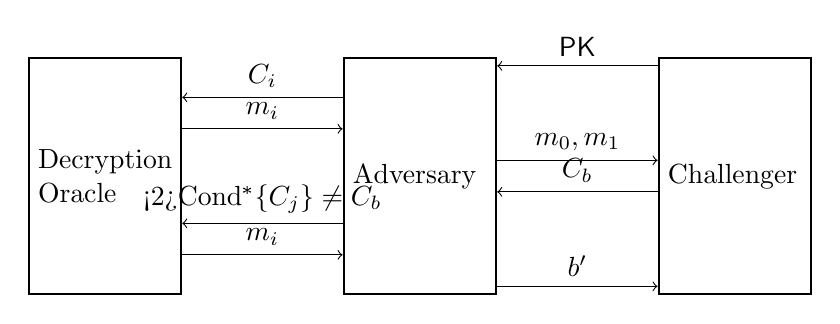
\begin{tikzpicture}
      \node(A)[draw, thick, text width = 1.7cm, minimum height = 3cm] at (0,0) {Adversary};
      \node(C)[draw, thick, text width = 1.7cm, minimum height = 3cm] at (4,0) {Challenger};
      \node(D)[draw, thick, text width = 1.7cm, minimum height = 3cm] at (-4,0) {Decryption Oracle};
      
      \path([yshift = 1.4cm]A.east) edge[<-] node[above]{$\PK$} ([yshift = 1.4cm]C.west);
      \path([yshift = 1cm]D.east) edge[<-] node[above]{$C_i$} ([yshift = 1cm]A.west);
      \path([yshift = 0.6cm]D.east) edge[->] node[above]{$m_i$} ([yshift = 0.6cm]A.west);
      \path([yshift = 0.2cm]A.east) edge[->] node[above]{$m_0, m_1$} ([yshift = 0.2cm]C.west);
      
      \path([yshift = -0.2cm]A.east) edge[<-] node[above]{$C_b$}([yshift = -0.2cm]C.west);
      \path([yshift = -0.6cm]D.east) edge[<-] node[above]{\alt<2>{Cond\footnote{$Dec(k_d, \{C_j\}) \not \in \{m_0,m_1\}$}}{$\{C_j\}\neq C_b$}} ([yshift = -0.6cm]A.west);
      \path([yshift = -1cm]D.east) edge[->] node[above]{$m_i$} ([yshift = -1cm]A.west);
      
      \path([yshift = -1.4cm]A.east) edge[->] node[above]{$b'$}([yshift = -1.4cm]C.west);
    \end{tikzpicture}
    
  \end{figure}
 
  {\color{blue} Advantage:} $Adv(\Adv) = |\PR[b = b'] - \frac{1}{2}|$.
\end{frame}
 
\begin{frame}{Type 3 pairings and DDH (SXDH) assumption}
  \begin{block}{Pairing}
    For three groups $(\G, \hat{\G}, \G_T)$ of prime order $p$ and $e: \G \times \hat{\G} \to \G_T$.
    %    \begin{enumerate}
    %    \item Bilinear: $e (A^{\lambda}\cdot B,  C) = e(A,C)^{\lambda} \cdot e(B, C)$ and $e(A, B^{\lambda}\cdot C) = e(A, B)^{\lambda} \cdot e(A, C)$.
    %    \item Non-degenerate: Non-trivial $A,B$ verify $e(A, B) \neq 1$.
    %    \end{enumerate}
    \begin{align*}
      e(A^{\lambda}, B) &= e(A, B^{\lambda}) & e(g,h) = 1 &\mbox{ iff } g=1 \vee h=1 
    \end{align*}
    \pause
    \begin{itemize}
    \item No comutable isomorphism between $\G$ and $\hat{\G}$.
      \pause
    \item Most efficient pairing configuration.
    \end{itemize}
  \end{block}
  \pause
  \begin{block}{DDH (SXDH) assumption}.
    $g \in \G$ and $a,b,c \sample \mathbb{Z}_p$
 
    \begin{itemize}
    \item DDH:
      $$\{g,g^a, g^b, g^{ab}\} \approx_c \{g, g^a, g^b, g^c\}.$$
    \item SXDH: DDH in $\G$ and $\hat{\G}$.
    \end{itemize}
  \end{block}
 
\end{frame}


\begin{frame}{State of the art}
  
  \begin{block}{Structure-Preserving Signature}
    \begin{itemize}
    \item \cite{DBLP:journals/iacr/AbeHO10} Sign a message $\vec{M} = (m_1, m_2, \dots, m_n) \in \hat{\G}^n$ with a signature $2\G + 5\hat{\G}$ under SXDH with asymmetric pairing.
    \end{itemize}
  \end{block}

  \pause

  \begin{block}{Structure-Preserving Encryption}
    \begin{itemize}
    \item \cite{DBLP:conf/asiacrypt/CamenischHKLN11} Ciphertext of a message $m \in \G$ consists of $4\G + 1 \G_T$ under DLIN with symmetric pairing and not verifiable.
    \end{itemize}
  \end{block}
    
\end{frame}

\end{section}

\begin{section}{Preliminaries}
  
\begin{frame}{Building blocks}
  \begin{block}{building blocks for our Structure-Preserving CCA and RCCA schemes:}
    \begin{enumerate}
    \item Groth-Sahai Proof System~\cite{DBLP:conf/eurocrypt/GrothS08}.
    \item Structure-Preserving Commitment.
    \end{enumerate}
  \end{block}
\end{frame}


\begin{frame}{Groth-Sahai Proof System}
  \begin{block}{Proof Instance: Pairing Product Equation (PPE)}
    \begin{align*}
      \prod^{n}_{j=1} e(\mathcal{A}_j, {\color{red}\mathcal{Y}_j}) \prod^{m}_{i=1}e({\color{red}\mathcal{X}_i}, \mathcal{B}_i)\prod^{m}_{i=1} \prod^{n}_{j=1}e({\color{red}\mathcal{X}_i}, {\color{red}\mathcal{Y}_j})^{\gamma_{i,j}} &= t_T
    \end{align*}
    Where for $i \in \{1, \dots, m\}$ and $j \in \{1, \dots, n\}$
    \begin{enumerate}
    \item ${\color{red}\mathcal{X}_i}$ variables in $\G$, ${\color{red}\mathcal{Y}_j}$ variables in $\hat{\G}$.
    \item $\mathcal{A}_j$ constants in $\G$, $\mathcal{B}_i$ constants in $\hat{\G}$, $t_T$ constant in $\G_T$. and $\gamma_{i,j}$ constant in $\mathbb{Z}_n$
    \end{enumerate}
  \end{block}
  
\end{frame}

\begin{frame}{Groth-Sahai Proof System}
%  \begin{block}{Framework}
%    \begin{itemize}
%    \item $\Setup(\lambda) \to CRS$
%    \item $\Prove(CRS, (x, w)) \to \pi$
%    \item $\Verif(CRS, (x,w), \pi) \to \{\True, \False\}$
%    \end{itemize}
%  \end{block}

  A NIWI proof system $(\Setup, \Prove, \Verif)$:
  \pause
  \begin{itemize}
  \item Prove pairing product equations.
    \pause
  \item {\color{blue}Operate in two modes}: Depending on the common reference string $CRS = (\vec{u}_1, \vec{u}_2, \hat{\vec{u}}_1, \hat{\vec{u}}_2) \in \G^2 \times \G^2 \times \hat{\G}^2 \times \hat{\G}^2$.
    \pause
  	\begin{itemize}
  	\item  {\color{blue}(Soundness setting)} Exists $\zeta, \hat{\zeta} \in \mathbb{Z}_p$ \st $\vec{u}_2 = \vec{u}_1^\zeta$ and $\hat{\vec{u}}_2 = \hat{\vec{u}}_1^{\hat{\zeta}}$. Using $\zeta, \hat{\zeta}$, we can 
          \begin{enumerate}
          \item Simulate a proof for false statement.
          \item Extract the witness from a valid proof.
          \end{enumerate}
          \pause
  	\item {\color{blue}(Witness-Indistinguishable (WI) setting)} $(\vec{u}_1, \vec{u}_2)$ and $(\hat{\vec{u}}_1,  \hat{\vec{u}}_2)$ are pairwise independent.
          \begin{enumerate}
          \item Cannot prove false statement
          \item Proofs using different valid witnesses are indistinguishable.
          \end{enumerate}
  	\end{itemize}
  \end{itemize}
  
%  \pause
%  \begin{block}{Example}
%    \begin{itemize}
%    \item $\Setup(\lambda)$:  $(\G, \hat{\G}, \G_T)$ of prime order $p > 2^\lambda$ with generators $(g,\hat{g}) \sample \G \times \hat{\G}$, $\vec{u}_1, \vec{u}_2 \sample \G^2$.
%    \item $\Prove(CRS, (x, w))$: 
%    \item $\Verif(CRS, (x,w), \pi) \to \{\True, \False\}$
%    \end{itemize}
%  \end{block}
\end{frame}





\begin{frame}{Strictly Structure-Preserving Commitment~\cite{DBLP:conf/eurocrypt/AbeKOT15}}

  Strictly Structure-Preserving Commitment $(\Setup, \Com, \Verif)$ satisfying \pause
%  \begin{block}{Framework}
%      \begin{itemize}
%      \item $\Setup(\lambda) \to \ck$: Generates commitment key $\ck$.
%      \item $\Com(\ck, m; \open) \to (\com,\open)$: Generates a commitment $\com$ \wrt the randomness $\open$.
%      \item $\Verif(\ck, m, \com, \open) \to \{True, False\}$: Outputs convinced or not.
%      \end{itemize}
%  \end{block}
%\end{frame}
%\begin{frame}{Strictly Structure-Preserving Commitment~\cite{DBLP:conf/eurocrypt/AbeKOT15}}
  \begin{block}{Properties}
    \begin{itemize}
      %    \item (Binding) No (PPT)adversary can produce $(m, m', \open, \open', \com)$ \st $\Verif(\ck, m, \com, \open) = \True$ and $\Verif(\ck, m', \com, \open') = \True$ and $m \neq m'$
      %    \item (Hiding)
    \item {\color{blue}(Correctness)} $\Verif(\ck, m, \Com(\ck, m; \open), \open) = \True$.
      \pause
    \item {\color{blue}(\textbf{Enhanced} Chosen-Message Target Collision Resistant (ECM-TCR))} Given $\com^*, m^*, \open^*$ a valid commitment. Hard to generate $(m, \open)$ \st
      \begin{align*}
        \Verif(\ck, m, \com^*, \open) &= \True \wedge (m, \open) \neq (m^*, \open^*)
      \end{align*}
    \item {\color{blue}(Stricly Structure-Preserving)} The commitment is also in the source group $\G$ or $\hat{\G}$.
    \end{itemize}
  \end{block}
\end{frame}



\end{section}

\begin{section}{Construction}

\end{section}

\begin{section}{Proof idea}

\end{section}
% 
%\begin{section}{Contributions}
%  \begin{frame}{Our contributions}
  \setbeamercolor{normal text}{fg=gray,bg=}
  \setbeamercolor{alerted text}{fg=black,bg=}
  \usebeamercolor{normal text}

  \begin{enumerate}
  \item\alert<+>{ Construction of an efficient Structure-Preserving Publicly Verifiable Encryption $16\times\G + 11\times\hat{\G}$ against $321\times\G$ [Abe \etal~2013].}
  \item\alert<+>{ Construction an efficient RCCA rerandomizable encryption scheme $29 \times\G + 20 \times\hat{\G}$ against $93\times\G$ under the DLIN assumption or $49\times\G +20 \times\hat{\G}$ under the SXDH assumption.~\cite{DBLP:conf/eurocrypt/ChaseKLM12} }.
  \end{enumerate}
\end{frame}

%\end{section}
% 
%\begin{section}{Preliminaries}
%  
\begin{frame}{Building blocks}
  \begin{block}{building blocks for our Structure-Preserving CCA and RCCA schemes:}
    \begin{enumerate}
    \item Groth-Sahai Proof System~\cite{DBLP:conf/eurocrypt/GrothS08}.
    \item Structure-Preserving Commitment.
    \end{enumerate}
  \end{block}
\end{frame}


\begin{frame}{Groth-Sahai Proof System}
  \begin{block}{Proof Instance: Pairing Product Equation (PPE)}
    \begin{align*}
      \prod^{n}_{j=1} e(\mathcal{A}_j, {\color{red}\mathcal{Y}_j}) \prod^{m}_{i=1}e({\color{red}\mathcal{X}_i}, \mathcal{B}_i)\prod^{m}_{i=1} \prod^{n}_{j=1}e({\color{red}\mathcal{X}_i}, {\color{red}\mathcal{Y}_j})^{\gamma_{i,j}} &= t_T
    \end{align*}
    Where for $i \in \{1, \dots, m\}$ and $j \in \{1, \dots, n\}$
    \begin{enumerate}
    \item ${\color{red}\mathcal{X}_i}$ variables in $\G$, ${\color{red}\mathcal{Y}_j}$ variables in $\hat{\G}$.
    \item $\mathcal{A}_j$ constants in $\G$, $\mathcal{B}_i$ constants in $\hat{\G}$, $t_T$ constant in $\G_T$. and $\gamma_{i,j}$ constant in $\mathbb{Z}_n$
    \end{enumerate}
  \end{block}
  
\end{frame}

\begin{frame}{Groth-Sahai Proof System}
%  \begin{block}{Framework}
%    \begin{itemize}
%    \item $\Setup(\lambda) \to CRS$
%    \item $\Prove(CRS, (x, w)) \to \pi$
%    \item $\Verif(CRS, (x,w), \pi) \to \{\True, \False\}$
%    \end{itemize}
%  \end{block}

  A NIWI proof system $(\Setup, \Prove, \Verif)$:
  \pause
  \begin{itemize}
  \item Prove pairing product equations.
    \pause
  \item {\color{blue}Operate in two modes}: Depending on the common reference string $CRS = (\vec{u}_1, \vec{u}_2, \hat{\vec{u}}_1, \hat{\vec{u}}_2) \in \G^2 \times \G^2 \times \hat{\G}^2 \times \hat{\G}^2$.
    \pause
  	\begin{itemize}
  	\item  {\color{blue}(Soundness setting)} Exists $\zeta, \hat{\zeta} \in \mathbb{Z}_p$ \st $\vec{u}_2 = \vec{u}_1^\zeta$ and $\hat{\vec{u}}_2 = \hat{\vec{u}}_1^{\hat{\zeta}}$. Using $\zeta, \hat{\zeta}$, we can 
          \begin{enumerate}
          \item Simulate a proof for false statement.
          \item Extract the witness from a valid proof.
          \end{enumerate}
          \pause
  	\item {\color{blue}(Witness-Indistinguishable (WI) setting)} $(\vec{u}_1, \vec{u}_2)$ and $(\hat{\vec{u}}_1,  \hat{\vec{u}}_2)$ are pairwise independent.
          \begin{enumerate}
          \item Cannot prove false statement
          \item Proofs using different valid witnesses are indistinguishable.
          \end{enumerate}
  	\end{itemize}
  \end{itemize}
  
%  \pause
%  \begin{block}{Example}
%    \begin{itemize}
%    \item $\Setup(\lambda)$:  $(\G, \hat{\G}, \G_T)$ of prime order $p > 2^\lambda$ with generators $(g,\hat{g}) \sample \G \times \hat{\G}$, $\vec{u}_1, \vec{u}_2 \sample \G^2$.
%    \item $\Prove(CRS, (x, w))$: 
%    \item $\Verif(CRS, (x,w), \pi) \to \{\True, \False\}$
%    \end{itemize}
%  \end{block}
\end{frame}





\begin{frame}{Strictly Structure-Preserving Commitment~\cite{DBLP:conf/eurocrypt/AbeKOT15}}

  Strictly Structure-Preserving Commitment $(\Setup, \Com, \Verif)$ satisfying \pause
%  \begin{block}{Framework}
%      \begin{itemize}
%      \item $\Setup(\lambda) \to \ck$: Generates commitment key $\ck$.
%      \item $\Com(\ck, m; \open) \to (\com,\open)$: Generates a commitment $\com$ \wrt the randomness $\open$.
%      \item $\Verif(\ck, m, \com, \open) \to \{True, False\}$: Outputs convinced or not.
%      \end{itemize}
%  \end{block}
%\end{frame}
%\begin{frame}{Strictly Structure-Preserving Commitment~\cite{DBLP:conf/eurocrypt/AbeKOT15}}
  \begin{block}{Properties}
    \begin{itemize}
      %    \item (Binding) No (PPT)adversary can produce $(m, m', \open, \open', \com)$ \st $\Verif(\ck, m, \com, \open) = \True$ and $\Verif(\ck, m', \com, \open') = \True$ and $m \neq m'$
      %    \item (Hiding)
    \item {\color{blue}(Correctness)} $\Verif(\ck, m, \Com(\ck, m; \open), \open) = \True$.
      \pause
    \item {\color{blue}(\textbf{Enhanced} Chosen-Message Target Collision Resistant (ECM-TCR))} Given $\com^*, m^*, \open^*$ a valid commitment. Hard to generate $(m, \open)$ \st
      \begin{align*}
        \Verif(\ck, m, \com^*, \open) &= \True \wedge (m, \open) \neq (m^*, \open^*)
      \end{align*}
    \item {\color{blue}(Stricly Structure-Preserving)} The commitment is also in the source group $\G$ or $\hat{\G}$.
    \end{itemize}
  \end{block}
\end{frame}



%\end{section}
% 
% 
% 
%\begin{section}{Construction of Structure-Preserving Publicly Verifiable Encryption}
%  \begin{frame}{Structure-Preserving Publicly Verifiable Encryption}
  \begin{block}{Framework}
    \begin{itemize}
    \item $\Setup(\lambda) \to \PPP$
    \item $\KeyGen(\PPP) \to (\PK, \SK)$
    \item $\Enc(\PPP, \PK, m) \to c$
    \item $\Dec(\PPP, \SK, c) \to m \mbox{ or } \bot$
    \item $\Verif(\PPP, \PK, c) \to \{\True, \False\}$
    \end{itemize}
  \end{block}

  \begin{block}{Some parameters}
    
    \begin{itemize}
    \item $\SK = (x_1, x_2)$.
    \item $\PK = (g_1, g_2, X = g_1^{x_1}g_2^{x_2}, \PPP_{SPC}, \vec{\ck}, CRS_{GS} = (\hat{\vec{u}}_1, \hat{\vec{u}}_2) \in \hat{\G}^2 \times \hat{\G}^2)$.
    \end{itemize}
    where $(g_1, g_2) \in \G^2$, $(x_1, x_2) \in \mathbb{Z}_p^2$ and $\exists \rho_u \in \mathbb{Z}_p$ such that $\hat{\vec{u}}_1 = \hat{\vec{u}}_2^{\rho_u}$.
  \end{block}
  
\end{frame}

\begin{frame}{Structure-Preserving Publicly Verifiable Encryption}
%  \begin{block}{CRS for the Groth-Sahai proof}
%  $(\hat{\vec{u}}_1, \hat{\vec{u}}_2) \in \hat{\G}^2 \times \hat{\G}^2$ and $\rho_u \in \mathbb{Z}_p$ which verifies $\hat{\vec{u}}_2 = \hat{\vec{u}}_1^{\rho_u}$. 
%  \end{block}
%   $CRS_{GS} = (\hat{\vec{u}}_1, \hat{\vec{u}}_2) \in \hat{\G}^2 \times \hat{\G}^2$ which verifies $\exists \rho_u \in \mathbb{Z}_p$ such that $\hat{\vec{u}}_1 = \hat{\vec{u}}_2^{\rho_u}$.
  \begin{block}{Details of the Encryption algorithm}
   
    \begin{itemize}
    \item Generate $\vec{C} = (C_0, C_1, C_2) = (MX^{\theta}, g_1^{\theta},  g_2^{\theta})$.
    \item $\Sig.\KeyGen(\PPP) \to (\SSK, \SVK)$.
    \item $\Com(\ck, \SVK) \to (\hat{\com}, \open)$.
    \item Compute $\hat{\vec{u}}_{\hat{\com}} = \hat{\vec{u}}_2 \cdot (1, \hat{\com}) \in \hat{\G}^2$.
    \item $\Prove(CRS_{\hat{\com}} = (\hat{\vec{u}}_1, \hat{\vec{u}}_{\com}), x = (C_1, C_2), w = \theta) \to \pi$ of the fact $\exists \chi$ such that $(C_1, C_2) = (g_1^\chi, g_2^\chi)$.
    \item $\Sig.\Sig(\SSK,(\vec{C},\pi)) \to \sigma$.
    \item Output the ciphertext $(\vec{C}, \pi, \SVK, \hat{\com}, \open, \sigma) \in \G^{16} \times \hat{\G}^{11}$.
    \end{itemize}

  \end{block}
\end{frame}


\begin{frame}{Proof intuitions}
  \begin{columns}
    \begin{column}{0.5\textwidth}
        \tiny
      \begin{figure}
        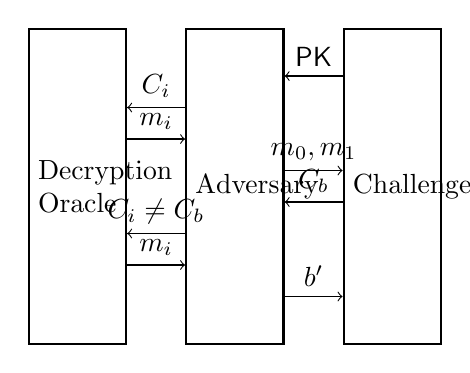
\begin{tikzpicture}
      \node(A)[draw, thick, text width = 1cm, minimum height = 4cm] at (0,0) {Adversary};
      \node(C)[draw, thick, text width = 1cm, minimum height = 4cm] at (2,0) {Challenger};
      \node(D)[draw, thick, text width = 1cm, minimum height = 4cm] at (-2,0) {Decryption Oracle};
      
      \path([yshift = 1.4cm]A.east) edge[<-] node[above]{$\PK$} ([yshift = 1.4cm]C.west);
      \path([yshift = 1cm]D.east) edge[<-] node[above]{$C_i$} ([yshift = 1cm]A.west);
      \path([yshift = 0.6cm]D.east) edge[->] node[above]{$m_i$} ([yshift = 0.6cm]A.west);
      \path([yshift = 0.2cm]A.east) edge[->] node[above]{$m_0, m_1$} ([yshift = 0.2cm]C.west);
      
      \path([yshift = -0.2cm]A.east) edge[<-] node[above]{$C_b$}([yshift = -0.2cm]C.west);
      \path([yshift = -0.6cm]D.east) edge[<-] node[above]{$C_i \neq C_b$} ([yshift = -0.6cm]A.west);
      \path([yshift = -1cm]D.east) edge[->] node[above]{$m_i$} ([yshift = -1cm]A.west);
      
      \path([yshift = -1.4cm]A.east) edge[->] node[above]{$b'$}([yshift = -1.4cm]C.west);
    \end{tikzpicture}
  \end{figure}
    \end{column}

    \begin{column}{0.5\textwidth}

      
      \tiny
      \alt<3->{{\color{red} $CRS_{GS} = (\hat{\vec{u}}_1, \hat{\vec{u}}_2 \cdot (1, \hat{\com}^{-1}))$ with $\hat{\vec{u}}_1 = \hat{\vec{u}}_2^{\rho_u}$}}{{\color{red} $CRS_{GS} = (\hat{\vec{u}}_1, \hat{\vec{u}}_2)$ with $\hat{\vec{u}}_1 = \hat{\vec{u}}_2^{\rho_u}$}}.
	
      Encryption
    \begin{itemize}
    \item Generate $\vec{C}^* = (C_0^*, C_1^*, C_2^*) = (\alt<4->{{\color{red}M_bC_1^{x_1}C_2^{x_2}}}{ M_bX^{\theta^*}}, g_1^{\alt<5->{{\color{red}\theta_1}}{\theta^*}},  g_2^{\alt<5->{{\color{red}\theta_2}}{\theta^*}})$.
    \item $\Sig.\KeyGen(\PPP) \to (\SSK^*, \SVK^*)$\visible<2->{{\color{red} Do this at beginning}}.
    \item $\Com(\ck, \SVK^*) \to (\hat{\com}^*, \open^*)$\visible<2->{{\color{red} Do this at beginning}}.
    \item Compute $\hat{\vec{u}}_{\hat{\com}} = \hat{\vec{u}}_2 \cdot (1, \hat{\com}) \in \hat{\G}^2$.	
    \item $\Prove(CRS_{\hat{\com}}= (\hat{\vec{u}}_1, \hat{\vec{u}}_{\hat{\com}}), x = (C_1^*, C_2^*), w = \theta^*) \to \pi^*$ of the fact $\exists \chi$ such that $(C_1^*, C_2^*) = (g_1^\chi, g_2^\chi)$.
    \item $\Sig(\SSK^*,(\vec{C}^*,\pi^*)) \to \sigma^*$.
    \item Output the ciphertext $(\vec{C}^*, \pi^*, \SVK^*, \hat{\com}^*, \open^*, \sigma^*) \in \G^{16} \times \hat{\G}^{11}$.
    \end{itemize}
    \end{column}

  \end{columns}
\end{frame}

%\end{section}
% 
%\begin{section}{Rerandomizable Encryption Scheme}
%  \begin{frame}{Rerandomizable encryption}

  %  \begin{block}{Details of the Encryption algorithm}
  %    \begin{itemize}
  %    \item Generate $\vec{C} = (C_0, C_1, C_2) = (MX^{\theta}, g_1^{\theta},  g_2^{\theta})$.
  %    \item $LHSPS.\KeyGen(\PPP) \to (\SSK, \SVK)$.
  %    \item $\Com(\ck, \SVK) \to (\com, \open)$.
  %    \item $\Prove(\PPP_{ABOProof}, x = (C_1, C_2), w = \theta, tag = \com) \to \pi$ of the fact $\exists \chi$ such that $(C_1, C_2) = (g_1^\chi, g_2^\chi)$.
  %    \item $LHSPS.\Sig(\SVK,((C_0,C_1,C_2, g),\pi)) \to \sigma_m$.
  %    \item $LHSPS.\Sig(\SVK,((X,g_1,g_2, 1),\pi)) \to \sigma_1$.
  %    \item $NIZK.\Prove(\PPP, m = (C_1, C_2), w = (\com,\pi)) \to \pi_{com}$
  %    \item $NIZK.\Prove(\PPP, m = (C_0,C_1,C_2,g), w = (\SVK, \sigma_m)) \to \pi_{\sigma_m}$
  %    \item $NIZK.\Prove(\PPP, m = (X,g_1,g_2,1), w = (\SVK, \sigma_1)) \to \pi_{\sigma_1}$
  %    \item Output the ciphertext $(\vec{C},\pi_{com}, \pi_{\sigma_m}, \pi_{\sigma_1}) \in \G^{39} \times \hat{\G}^{20}$.
  %    \end{itemize}
  % 
  %  \end{block}


  \begin{columns}
    \begin{column}{0.5\textwidth}
      \tiny
      Structure-Preserving Publicly Verifiable Encryption 
      \begin{itemize}
      \item Generate $\vec{C} = (C_0, C_1, C_2) = (MX^{\theta}, g_1^{\theta},  g_2^{\theta})$.
      \item $\Sig.\KeyGen(\PPP) \to (\SSK, \SVK)$.
      \item $\Com(\ck, \SVK) \to (\com, \open)$.
      \item $\Prove(\PPP_{ABOProof}, x = (C_1, C_2), w = \theta, tag = \com) \to \pi$ of the fact $\exists \chi$ such that $(C_1, C_2) = (g_1^\chi, g_2^\chi)$.
      \item $\Sig(\SSK,(\vec{C},\pi)) \to \sigma$.
      \item Output the ciphertext $(\vec{C}, \pi, \SVK, \com, \open, \sigma) \in \G^{16} \times \hat{\G}^{11}$.
      \end{itemize}

    \end{column}

    \begin{column}{0.5\textwidth}
      \tiny
      RCCA encryption 
      \begin{itemize}
      \item Generate $\vec{C} = (C_0, C_1, C_2) = (MX^{\theta}, g_1^{\theta},  g_2^{\theta})$.
      \item $LHSPS.\KeyGen(\PPP) \to (\SSK, \SVK)$.
      \item $\Com(\ck, \SVK) \to (\com, \open)$.
      \item $\Prove(\PPP_{ABOProof}, x = (C_1, C_2), w = \theta, tag = \com) \to \pi$ of the fact $\exists \chi$ such that $(C_1, C_2) = (g_1^\chi, g_2^\chi)$.
      \item {\color{red}$LHSPS.\Sig(\SSK,((C_0,C_1,C_2, g),\pi)) \to \sigma_m$.}
      \item {\color{red}$LHSPS.\Sig(\SSK,((X,g_1,g_2, 1),\pi)) \to \sigma_1$.}
        {\color{blue}
        \item $NIZK.\Prove(\PPP, m = (C_1, C_2), w = (\com,\pi)) \to \pi_{com}$
        \item $NIZK.\Prove(\PPP, m = (\SVK), w = (\com, \open)) to \pi_{\SVK}$
        \item $NIZK.\Prove(\PPP, m = (C_0,C_1,C_2,g), w = (\SVK, \sigma_m)) \to \pi_{\sigma_m}$
        \item $NIZK.\Prove(\PPP, m = (X,g_1,g_2,1), w = (\SVK, \sigma_1)) \to \pi_{\sigma_1}$
        }
        
      \item Output the ciphertext $(\vec{C},\pi_{com},\pi_{\SVK}, \pi_{\sigma_m}, \pi_{\sigma_1}) \in \G^{39} \times \hat{\G}^{20}$.
      \end{itemize}
 
    \end{column}
  \end{columns}
\end{frame}

%\end{section}
% 
%\begin{section}{Conclusion}
%  %\begin{frame}{Comparison}
%  \begin{enumerate}
%  \item Structure-Preserving Publicly Verifiable encryption $321\times\G$ by Abe \etal $\Rightarrow$ $16\times\G + 11\times\hat{\G}$
%  \item RCCA rerandomizable encryption $93\times\G$ or $49\times\G+20\times\hat{\G}$ $\Rightarrow$ $39\times\G + 20 \times\hat{\G}$
%  \end{enumerate}
%\end{frame}
% 
%\begin{frame}{Future work}
%  
%  \setbeamercolor{normal text}{fg=gray,bg=}
%  \setbeamercolor{alerted text}{fg=black,bg=}
%  \usebeamercolor{normal text}
%  
%  \begin{enumerate}
%  \item \alert<+>{Computational? Statistical?}
%  \item \alert<+>{More efficient?}
%  \end{enumerate}
%\end{frame}

\begin{frame}{Conclusion}
  \begin{block}{Future Works}
    \begin{itemize}
    \item Smaller ciphertext for rerandomization encryption scheme.
    \item Larger family of homomorphisms.
    \end{itemize}
  \end{block}
  \pause
  \begin{figure}
  \centering
  
\includegraphics[scale = 0.3]{./images/questions.png}
  \end{figure}
\end{frame}

%\end{section}

\backupbegin
\begin{frame}[plain, allowframebreaks,noframenumbering]
    \frametitle{References}
    \bibliographystyle{apalike}
    {\tiny \bibliography{presentation}}
\end{frame}
\backupend

\end{document}


